\begin{figure*}[t]
\centering
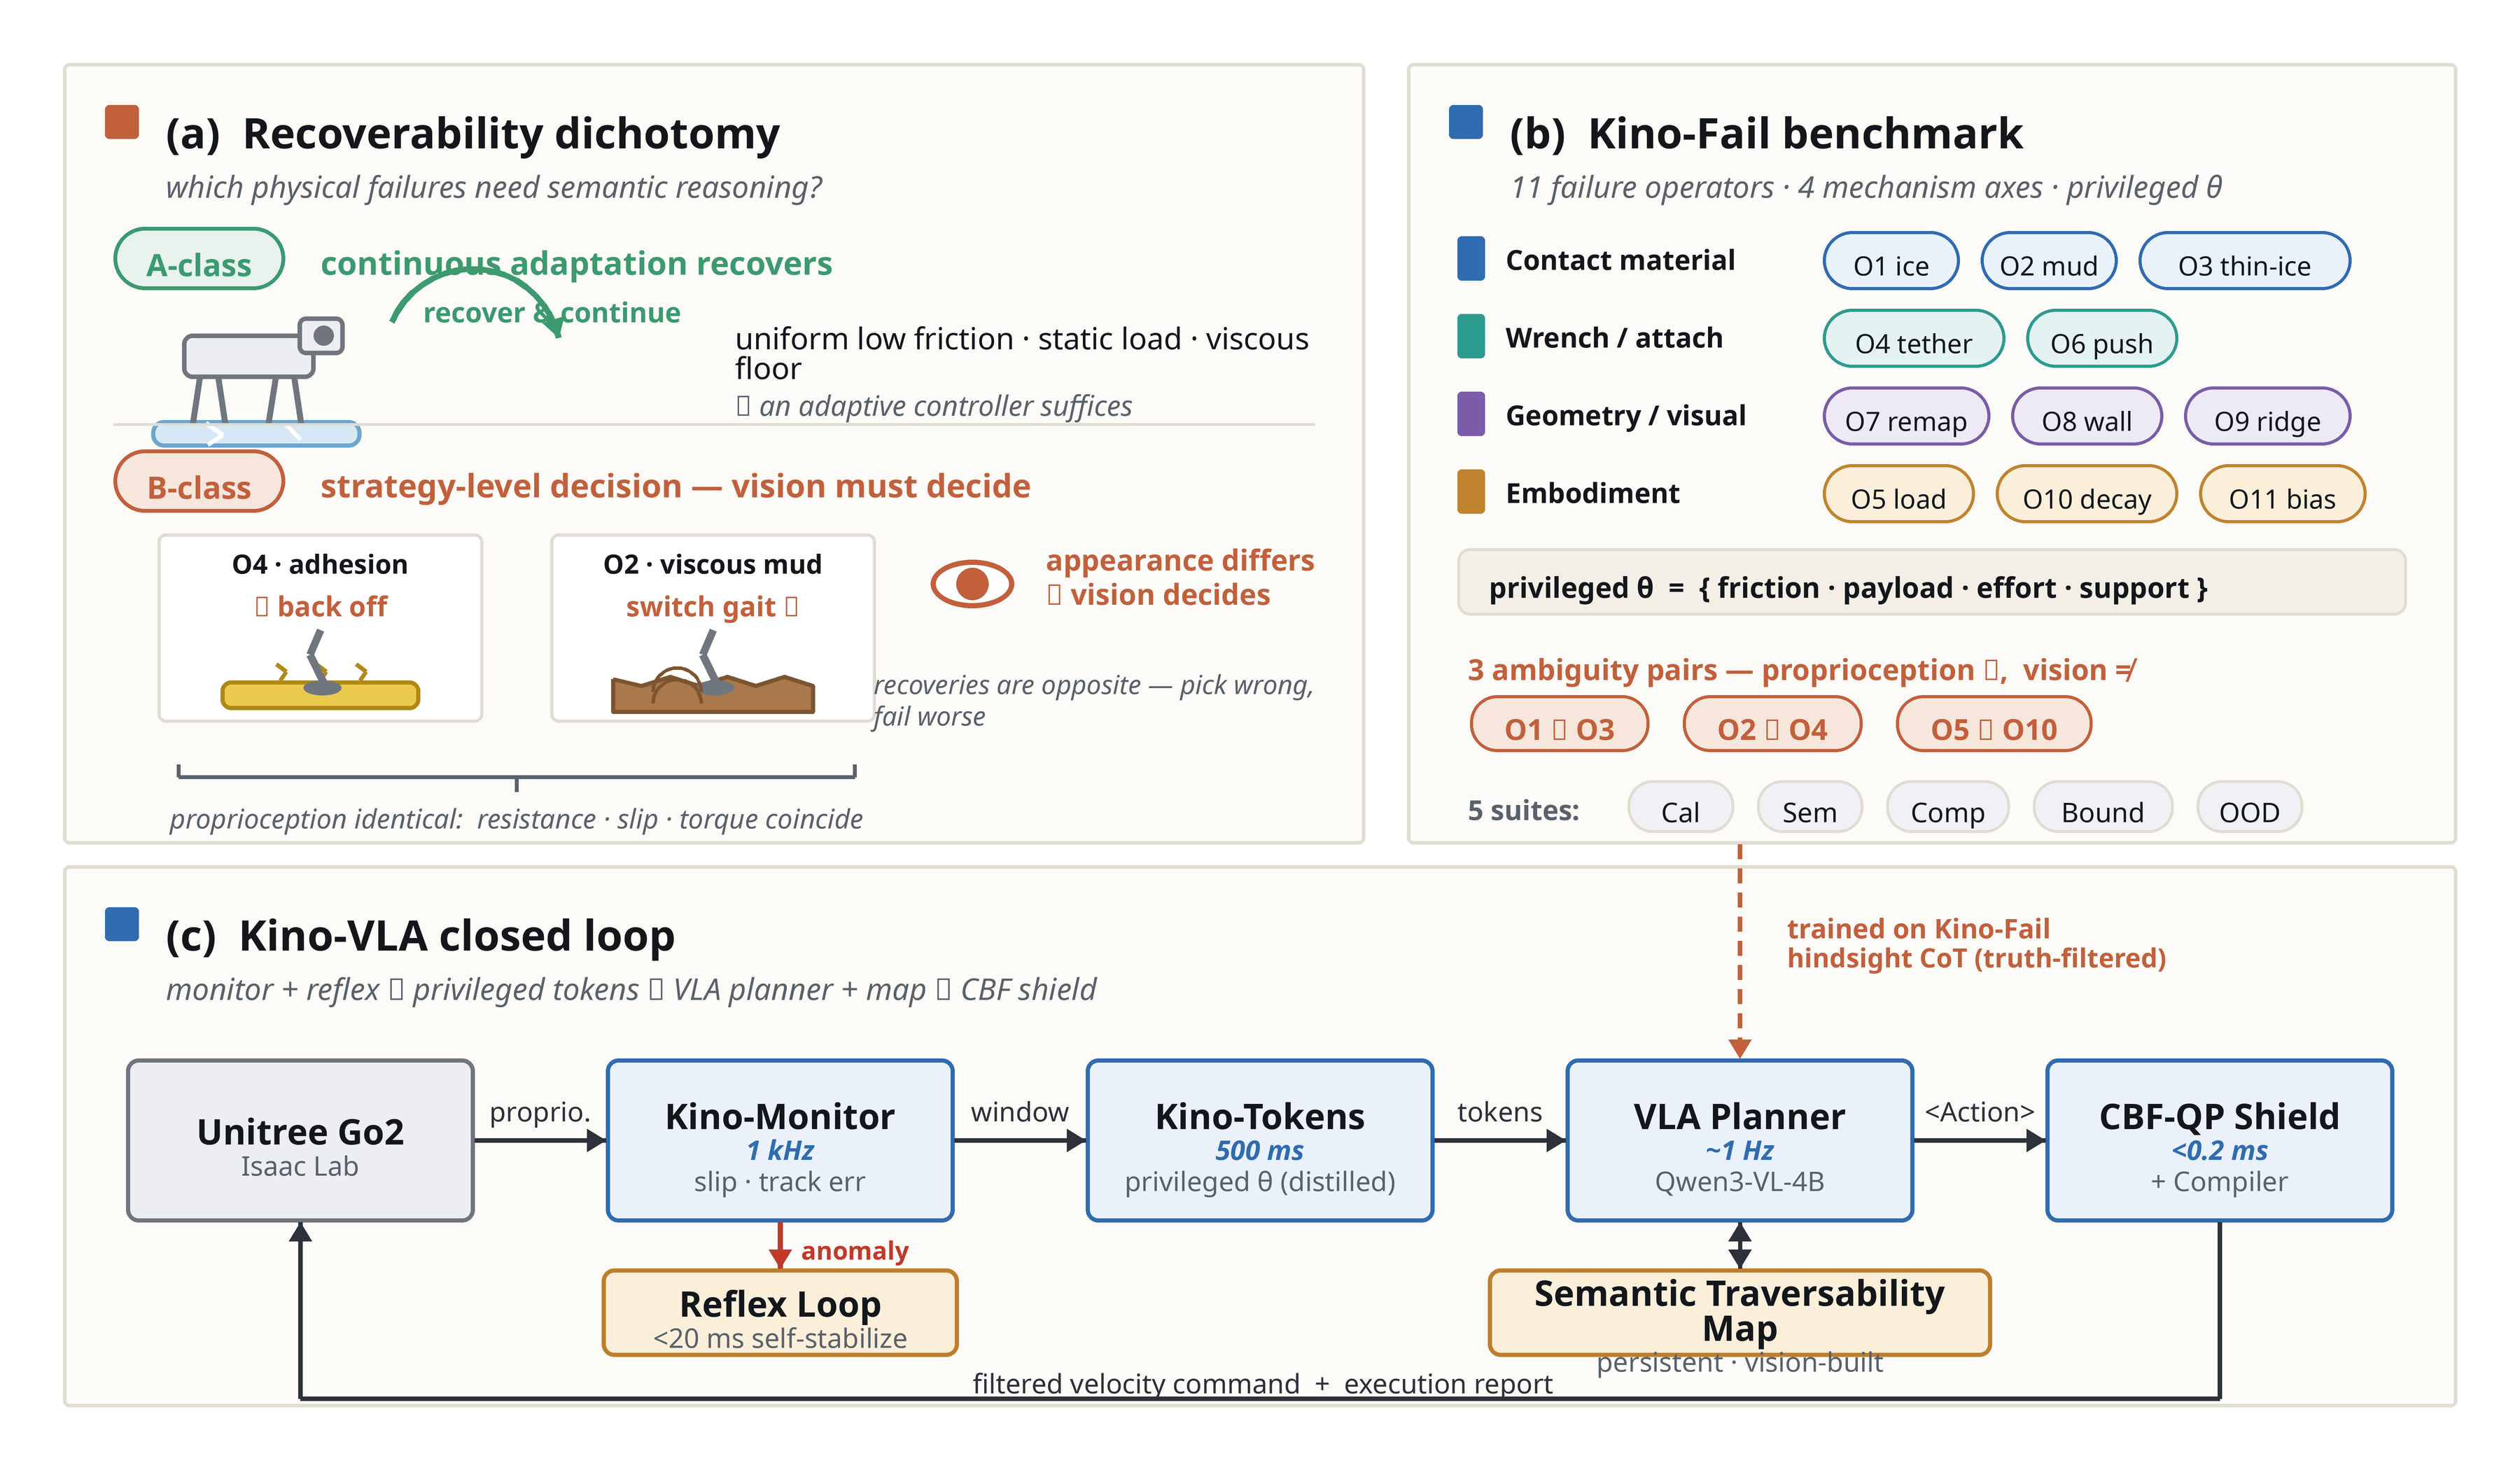
\includegraphics[width=\textwidth]{fig1_framework.png}
\iffalse  %% original TikZ source preserved below; figure is now rendered as fig1_system.png
\begin{tikzpicture}[
  font=\footnotesize,
  layer/.style={rectangle, rounded corners=2pt, draw=black!70, fill=blue!6,
                align=center, minimum height=13mm, text width=25mm, inner sep=3pt},
  plant/.style={rectangle, rounded corners=2pt, draw=black!75, fill=black!10,
                align=center, minimum height=13mm, text width=17mm, inner sep=3pt},
  aux/.style={rectangle, rounded corners=2pt, draw=black!55, fill=orange!8,
              align=center, minimum height=10mm, text width=25mm, inner sep=3pt},
  lab/.style={align=center, font=\scriptsize, text=black!65},
  fwd/.style={-{Latex[length=2mm,width=1.6mm]}, thick, black!80},
  fast/.style={-{Latex[length=2mm,width=1.6mm]}, line width=1pt, red!75!black},
  distill/.style={-{Latex[length=2mm,width=1.6mm]}, dashed, black!55},
  couple/.style={-{Latex[length=2mm,width=1.6mm]}, densely dotted, line width=0.9pt, orange!85!black},
]
% main forward pipeline
\node[plant] (robot) {Unitree Go2\\\textit{Isaac Lab}};
\node[layer, right=7mm of robot] (mon) {\textbf{Kino-Monitor}\\\textit{1\,kHz}\\slip, tracking err.};
\node[layer, right=7mm of mon] (tok) {\textbf{Kino-Tokens}\\\textit{500\,ms}\\1D-CNN $+$ Perceiver};
\node[layer, right=7mm of tok] (vla) {\textbf{VLA Planner}\\\textit{$\sim$1\,Hz}\\Qwen3-VL-4B $+$ LoRA};
\node[layer, right=7mm of vla] (cbf) {\textbf{CBF-QP Shield}\\$+$ Compiler};
\draw[fwd] (robot) -- node[lab,above]{proprio.} (mon);
\draw[fwd] (mon) -- node[lab,above]{window} (tok);
\draw[fwd] (tok) -- node[lab,above]{tokens} (vla);
\draw[fwd] (vla) -- node[lab,above]{\texttt{<Action>}} (cbf);
% privileged distillation (training-time supervision)
\node[aux, above=7mm of tok] (theta) {privileged physics $\theta$\\\textit{(simulator truth)}};
\draw[distill] (theta) -- node[lab,right,pos=0.45]{distill} (tok);
% mu-hat coupling, over the top
\draw[couple] (tok.north) to[out=50,in=130] node[lab,above]{$\hat\mu$ friction bound} (cbf.north);
% reflex fast loop
\node[aux, below=8mm of mon] (reflex) {\textbf{Reflex Loop}\\\textit{$<$20\,ms self-stabilize}};
\draw[fast] (mon) -- node[lab,right,pos=0.45]{anomaly} (reflex);
\draw[fast] (reflex.west) to[out=180,in=-90] ([xshift=-2mm]robot.south);
% semantic map + RGB-D
\node[aux, below=8mm of vla] (map) {\textbf{Semantic}\\\textbf{Traversability Map}};
\draw[{Latex[length=2mm]}-{Latex[length=2mm]}, thick, black!70] (vla) -- (map);
\node[lab, left=6mm of map] (rgbd) {RGB-D\\\textit{30\,Hz}};
\draw[fwd] (rgbd) -- (map);
% big feedback loop: cbf -> robot
\draw[fwd] (cbf.south) -- ([yshift=-24mm]cbf.south)
  -- node[lab,below]{filtered $v_{\mathrm{cmd}}^{\star}$ \ $+$ \ Execution Report} ([yshift=-24mm]robot.south)
  -- ([xshift=2mm]robot.south);
\end{tikzpicture}
\fi
\caption{\textbf{The \kinovla{} framework.} \textbf{(a) Recoverability dichotomy.}
A-class failures (uniform low friction, a static load, a viscous floor) are
recovered by continuous adaptation; B-class failures need a strategy-level
decision. An adhesive trap (O4) and viscous mud (O2) produce \emph{identical}
proprioception---resistance, slip, and torque coincide---yet demand opposite
recoveries (back off vs.\ switch gait), so only vision can decide. \textbf{(b)
\kinofail{} benchmark.} Eleven parameterized failure operators on four mechanism
axes, each exposing a privileged ground-truth parameter $\theta$ (friction,
payload, effort, support); three constructively matched ambiguity pairs
(O1$\leftrightarrow$O3, O2$\leftrightarrow$O4, O5$\leftrightarrow$O10) on which
proprioception coincides; and five evaluation suites (Cal, Sem, Comp, Bound, OOD).
\textbf{(c) Closed loop} on a physically simulated Unitree Go2. A \mbox{1\,kHz}
Kino-Monitor and a millisecond reflex keep the robot upright; a \kinotokens{}
extractor distills a \mbox{500\,ms} proprioceptive window into the planner under
privileged-physics supervision; the \mbox{$\sim$1\,Hz} VLA planner---trained on the
truth-filtered hindsight chain-of-thought data from (b)---attributes the failure,
emits one recovery primitive, and reads and writes a persistent semantic
traversability map, while the CBF-QP shield projects every primitive onto a
provably safe set ($<$\mbox{0.2\,ms}) before it is compiled to a velocity command.}
\label{fig:system}
\end{figure*}
